\documentclass{scrartcl}

\usepackage{amsmath}
\usepackage{siunitx}
\usepackage{mhchem}
\usepackage{booktabs}
\usepackage{graphicx}

\usepackage{pgfplots}
\pgfplotsset{compat = newest}


\begin{document}





\tableofcontents



%%%%%%%%%%%%%%%%%%%%%%%%%%%%%%%%%%%%%%%%%%%%%%%%%%%%%%%%%%%%%%%%%%%%%%%%%%%%%%%%
%%%%%%%%%%%%%%%%%%%%%%%%%%%%%%%%%%%%%%%%%%%%%%%%%%%%%%%%%%%%%%%%%%%%%%%%%%%%%%%%
%%%%%%%%%%%%%%%%%%%%%%%%%%%%%%%%%%%%%%%%%%%%%%%%%%%%%%%%%%%%%%%%%%%%%%%%%%%%%%%%

\section{Introduction}
In aquaponic systems, it is commonly reported that certain plant nutrients are lacking. Furthermore, it is oftentimes observed that some compounds reach a concentration plateau even though they are continuously supplied to the system. Thus, there has to be a constraint that is controlling the concentration of these compounds in the water.\\
If microbial uptake is neglected, two potential constraints are
\begin{itemize}
	\item the chemical satiation concentration
	\item nutrient depletion via water exchange
\end{itemize}
. It was found that the satiation concentrations of most of the plant nutrients are about three orders of magnitude higher than the concentrations observed in aquaponic systems. Thus, the water exchange might be what the right thing to look for in some cases.



%%%%%%%%%%%%%%%%%%%%%%%%%%%%%%%%%%%%%%%%%%%%%%%%%%%%%%%%%%%%%%%%%%%%%%%%%%%%%%%%
%%%%%%%%%%%%%%%%%%%%%%%%%%%%%%%%%%%%%%%%%%%%%%%%%%%%%%%%%%%%%%%%%%%%%%%%%%%%%%%%
%%%%%%%%%%%%%%%%%%%%%%%%%%%%%%%%%%%%%%%%%%%%%%%%%%%%%%%%%%%%%%%%%%%%%%%%%%%%%%%%



\section{Equations}

%%%%%%%%%%%%%%%%%%%%%%%%%%%%%%%%%%%%%%%%%%%%%%%%%%%%%%%%%%%%%%%%%%%%%%%%%%%%%%%%

\subsection{General considerations}
In general, the mass balance of an aquaculture system can be described considering the mass inputs $m_{in}$ and outputs $m_{out}$.

\begin{align}
	m_{acc} = m_{in} - m_{out}
	\label{eq1}
\end{align}

Depending on the values of $M_{in}$ and $m_{out}$ the resulting scenarios in terms of the mass $m_{acc}$ of a compound in the system are

\begin{itemize}
	\item $m_{in} > m_{out}$: Accumulation
 	\item $m_{in} = m_{out}$: Balance
 	\item $m_{in} < m_{out}$: Depletion
\end{itemize}

The accumulation rate over time can be described as 

\begin{align}
	\Delta m_{acc} = \frac{dV_{tot}c}{dt} = V_{tot}\frac{dc}{dt}
	\label{eq2}
\end{align}

, due to the constant volume $V_{tot}$ of the system. We assume that a substance (for instance a nutrient) is added continuously to the system at a constant mass. Thus, we assume a constant percentage water exchange of the total system volume, a constant mass input of feed and other substances. We can then write

\begin{align}
	V_{tot}\frac{dc}{dt} = Q_{in}c_{in} - Q_{out}c_{out}
	\label{eq3}
\end{align}

, with $Q_{in}$ and $Q_{out}$ describing the exchange volume per day and thus a volume flow per time unit and $c_{in}$ and $c_{out}$ as the concentration of the substance in the liquid entering or leaving the system, respectively. 



%%%%%%%%%%%%%%%%%%%%%%%%%%%%%%%%%%%%%%%%%%%%%%%%%%%%%%%%%%%%%%%%%%%%%%%%%%%%%%%%

\subsection{Scenario 1: Accumulation}
Considering a system with a water discharge of $0\%$, which would be the case if only evaporation water was replaced, Equation \ref{eq3} would be simplified to a constant mass input:

\begin{align}
	V_{tot}\frac{dc}{dt} = Q_{in}c_{in}	
	\label{eq3.1}
\end{align}

The constant input would eventually lead to a linear increase in the concentration of the targeted substance.


%%%%%%%%%%%%%%%%%%%%%%%%%%%%%%%%%%%%%%%%%%%%%%%%%%%%%%%%%%%%%%%%%%%%%%%%%%%%%%%%

\subsection{Scenario 2: Balance}
The starting point of the inflow-outflow mass balance is Equation \ref{eq3}. Because we are replacing the amount of water that we remove with the same amount of exchange water, we can write

\begin{align}
	Q_{in} = Q_{out} = Q
	\label{eq4}
\end{align}

. We can then substitute equation \ref{eq4} into equation \ref{eq3}, divide by $Q$ and obtain

\begin{align}
	\frac{V_{tot}}{Q} \frac{dc}{dt} = c_{in} - c_{out}
\end{align}

. Eventually, this equation can be integrated and rearranged with the following steps (see also Howe et al., Principles of Water Treatment).

\begin{align}
	\frac{Q}{V_{tot}} \int_{0}^{t} dt = \int_{0}^{c} \frac{dc}{c_{in} - c_{out}} 
\end{align}

\begin{align}
	\frac{1}{-1}\ln|c_{in} - c_{out}|_{0}^{c} = \frac{Q}{V}t
\end{align}

\begin{align}
	-\ln|c_{in} - c_{out}|-(-\ln|c_{in} - c_{out}|) = \frac{Q}{V}t
\end{align}

\begin{align}
	-\ln(c_{in} - c_{out})+\ln(c_{in}) = -\frac{Q}{V}t
\end{align}

\begin{align}
	\ln (\frac{c_{in}-c_{out}}{c_{in}}) = -\frac{Q}{V}t
\end{align}

\begin{align}
	c_{in} - c_{out} = c_{in} \cdot \exp^{-\frac{Q}{V}t}
\end{align}

\begin{align}
	1 - \frac{c_{out}}{c_{in}} = \exp^{-\frac{Q}{V}t}
\end{align}

\begin{align}
	\frac{c_{out}}{c_{in}} = 1 - \exp^{-\frac{Q}{V}t}
	\label{eq13}
\end{align}

The expression $\frac{Q}{V}$ in the equation is denoting for the \textbf{hydraulic retention time (HRT)}

\begin{align}
	\frac{Q}{V} = \tau
	\label{eq14}
\end{align}

, so that equation \ref{eq14} can be substituted into \ref{eq13}, resulting in 

\begin{align}
	\frac{c_{out}}{c_{in}} = 1 - \exp^{-\frac{t}{\tau}}
	\label{eq15}
\end{align}

. Equation \ref{eq15} can now be rearranged and gives

\begin{align}
	c_{out} = c_{in} (1 - \exp^{-\frac{t}{\tau}})
	\label{eq16}
\end{align}

. This model is generally known as the \textbf{Continuous Flow Stirred Tank Reactor (CFSTR)} model and is widely used in the field of chemical engineering. As shown in Figure \ref{fig1}, the model approaches 1 for $\lim_{t \to \infty}f(t)$.\\
%
%
%
%%%%%%%%%%%%%%%%%%%%%%%%%%%%%%%%%%%%%%%%%%%%%%%%%%%%%%%%%%%%%%%%%%%%%%%%%%%%%%%%
%
\begin{figure}
	\centering
	\begin{tikzpicture}	
	\begin{axis}[
	xlabel = $t$
	,ylabel = ${c_{out}}$
	%,y label style={rotate=3*90}
	]
		\addplot[domain=0:10] {1-e^-x};
		\addplot[domain=0:10,dashed] {1};
%		\addplot[domain=0:10, color=red, dashed] {2*(1-e^-x)};
%		\addplot[domain=0:10, color=red] {2};
	\end{axis}
	
	\end{tikzpicture}
	\caption{Asymptotic behaviour of the CFSTR model for $\lim_{t \to \infty}f(t)$.}
	\label{fig1}
\end{figure}
%
%%%%%%%%%%%%%%%%%%%%%%%%%%%%%%%%%%%%%%%%%%%%%%%%%%%%%%%%%%%%%%%%%%%%%%%%%%%%%%%%
%
\subsubsection{Time until steady state}
The time until a steady state in terms of the concentration is reached can be calculated as follows

\begin{align}
	\frac{c_{out}}{c_{in}} = 0.95 = 1 - \exp^{-\frac{t}{\tau}}\\
	\exp^{-\frac{t}{\tau}} = 1 - 0.95\\
	-\frac{t}{\tau} = \ln{0.05} = -3\\
	t_{95\%} = 3\tau
\end{align}

, with 95\% of the maximum concentration possible reached. The result shows, that it takes three times the retention time to reach this state. To come closer to the actual steady state where no change in concentration is expected to take place any more, the value for 99\%  of the maximum concentration is calculated.

\begin{align}
	\frac{c_{out}}{c_{in}} = 0.99 = 1 - \exp^{-\frac{t}{\tau}}\\
	\exp^{-\frac{t}{\tau}} = 1 - 0.99\\
	-\frac{t}{\tau} = \ln{0.01} = -4.6\\
	t_{99\%} = 4.6\tau
\end{align}

As can be seen, the maximum concentration is reached after 4.6 times the retention time.



\subsubsection{Substance losses over time}
To calculate the total loss of a substance over time in terms of mass, Equation \ref{eq16} can be integrated.


\begin{align}
	c_{out} = \int_{0}^{t} c_{in}(1 - \exp^{-\frac{t}{\tau}})\\
	c_{out} = c_{in}\int_{0}^{t} 1 - \exp^{-\frac{t}{\tau}}\\
	m_{out} = c_{in} V_{out} \int_{0}^{t} 1 - \exp^{-\frac{t}{\tau}}\\
	m_{out} = c_{in} V_{out} + \tau \cdot \exp^{-\frac{t}{\tau}} + c
\end{align}


\section{Input routes of substances}
The input routes of substances into aquaculture systems are 
\begin{enumerate}
	\item Source water
	\item Fish feed
	\item "Auxiliary substances" for water management
\end{enumerate}
. The input concentration $c_{in}$ can therefore be rewritten as

\begin{align}
	c_{in} = \frac{m_{in}}{V_{in}} = \frac{m_{w} + m_{f} + m_{a}}{V_{\ce{in}}}
\end{align}

, with $m_{w}$, $m_{f}$ and $m_{a}$ denoting for the nutrient mass supplied by water, feed and auxiliary substances, respectively.\\



%It is usually stated that the main proportion of nutrients enters the system via the fish feed. However, when having a closer look at the actual contribution of the feed and water to the total daily input (see \ref{figure1}), it becomes obvious that this claim is actually lacking any basis. The variables controlling the proportion of the nutrient that is provided by either feed or source water are the stocking density (and thus the biomass), the feeding rate, the concentration and mass fraction of the nutrient in the water and the feed, respectively, and the water exchange rate.\\





%%%%%%%%%%%%%%%%%%%%%%%%%%%%%%%%%%%%%%%%%%%%%%%%%%%%%%%%%%%%%%%%%%%%%%%%%%%%%%%%

%\begin{figure}
%	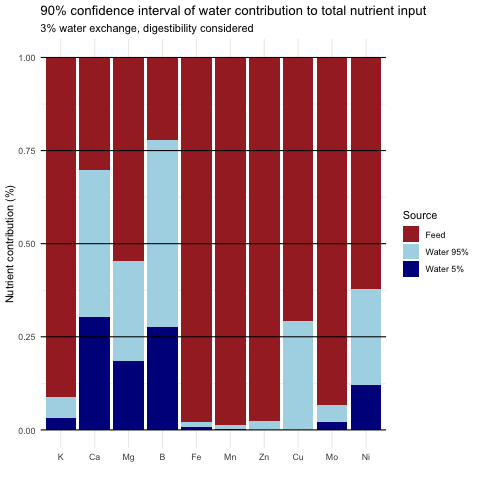
\includegraphics{plots/nutrientContribution.png}
%	\caption{Percentage of plant nutrients originating from fish feed and source water under the assumption that 3\% of the system water evaporated and was replaced by tap water (no nutrient outflow). Light blue color indicates the 90\% confidence interval of the corresponding concentrations in tap water. Tap water data obtained from 26 municipal tap water suppliers from 12 countries around the world. Average nutrient composition of 16 commercial fish feeds was used, regardless the fish species. Nutrient digestibility and retention in fish was considered, assuming an apparent digestibility of 50\% for each compound.}
%	\label{fig2}
%\end{figure}





%%%%%%%%%%%%%%%%%%%%%%%%%%%%%%%%%%%%%%%%%%%%%%%%%%%%%%%%%%%%%%%%%%%%%%%%%%%%%%%%
	
%\begin{table}[hbt]
%\centering
%  \caption{Model inputs and descriptions.}
%  \vspace{5mm}
%	\begin{tabular}{lcc}

%\toprule
% Abbreviation & Unit & Description\\
%\midrule
    
%$V_{tot}$ & \si{\liter} & Total volume of system\\
%$V_{r}$ & \si{\liter} & Rearing volume of system\\
%$V_{ex}$ & \si{\liter\per\day} & Volume of daily exchanged water\\
%$\rho_{fish}$ & \si{\kilo\gram\per\cubic\meter} & Stocking density of fish\\
%$m_{fish}$ & \si{\kilo\gram} & Total biomass of fish in the system\\
%$m_{feed}$ & \si{\kilo\gram\per\day} & Total mass of feed fed daily\\
%$m_{NUT}$ & \si{\milli\gram\per\day} & Daily mass input of nutrient\\
%$r_{ex}$ & \si{\percent\per\day} & Daily water exchange rate\\
%$r_{feed}$ & \si{\percent\per\day} & Daily feeding rate\\
%$c_{NUT, \ce{H2O}}$ & \si{\milli\gram\per\liter} & Concentration of compound in system water\\
%$c_{in}$ & \si{\milli\gram\per\liter} & Concentration of compound in source water\\
%$\omega$ & \si{\milli\gram\per\kilo\gram} & Mass fraction of compound in feed\\
%\bottomrule

%	\end{tabular}
%\end{table}





%%%%%%%%%%%%%%%%%%%%%%%%%%%%%%%%%%%%%%%%%%%%%%%%%%%%%%%%%%%%%%%%%%%%%%%%%%%%%%%%
%%%%%%%%%%%%%%%%%%%%%%%%%%%%%%%%%%%%%%%%%%%%%%%%%%%%%%%%%%%%%%%%%%%%%%%%%%%%%%%%
%%%%%%%%%%%%%%%%%%%%%%%%%%%%%%%%%%%%%%%%%%%%%%%%%%%%%%%%%%%%%%%%%%%%%%%%%%%%%%%%

%\section{Assumptions}
%Let it be assumed that the water in the system contains a concentration $c_{NUT, \ce{H2O}}$ of a nutrient. On a daily base, the amount $m_{NUT, feed}$ is introduced to the system via feed. The additional nutrients are homogeneously dissolved in the system water, thus adding $\frac{m_{NUT, feed}}{V_{tot}} = c_{feed}$ to the system. The resulting concentration is $c + c_{feed} = c_{tot}$. For the water exchange, a proportion of the system water that is given by $r_{ex}V_{tot} = V_{ex}$ is removed, resulting in the mass $m_{ex} = c_{tot}V_{ex}$ leaving the system. The removed water is then replaced by tap water with the nutrient concentration $c_{NUT, \ce{H2O}}$.\\
%The initial assumptions used for the creation of \ref{figure1} and for further calculations are shown in \ref{tab:assumptions}. These values are partly taken from literature.\\
%The described behaviour can be modelled using a \textbf{Continuous Flow Stirred Tank Reactor (CFSTR)} model with stepwise addition of a conservative tracer.





%%%%%%%%%%%%%%%%%%%%%%%%%%%%%%%%%%%%%%%%%%%%%%%%%%%%%%%%%%%%%%%%%%%%%%%%%%%%%%%%

%\begin{table}[!h]
%\centering
%  \caption{Initial assumptions.}
%  \label{tab:assumptions}
%  \vspace{5mm}
%	\begin{tabular}{lc}

%\toprule
% Abbreviation & Assumptions\\
%\midrule
    
%$V_{tot}$ & \SI{15000}{\liter}\\
%$V_{r}$ & \SI{10000}{\liter}\\
%$V_{ex}$ & \SI{4500}{\liter\per\day}\\
%$\rho_{fish}$ & \SI{25}{\kilo\gram\per\cubic\meter}\\
%$m_{fish}$ & \SI{250}{\kilo\gram}\\
%$m_{feed}$ & \SI{5}{\kilo\gram\per\day}\\
%$r_{ex}$ & \SI{3}{\percent\per\day}\\
%$r_{feed}$ & \SI{2}{\percent\per\day}\\
%\bottomrule

%	\end{tabular}
%\end{table}


\end{document}